\documentclass[conference]{IEEEtran}
% \IEEEoverridecommandlockouts
% The preceding line is only needed to identify funding in the first footnote. 
% If that is unneeded, please comment it out.

\usepackage{cite}
\usepackage{amsmath,amssymb,amsfonts}
\usepackage{algorithmic}
\usepackage{graphicx}
\usepackage{textcomp}
\usepackage{xcolor}
\usepackage{url}

\def\BibTeX{{\rm B\kern-.05em{\sc i\kern-.025em b}\kern-.08em
    T\kern-.1667em\lower.7ex\hbox{E}\kern-.125emX}}

\begin{document}

\title{Kingdomino: Enter the Virtual World}

\author{\IEEEauthorblockN{Hai Duong, Tran}
    \IEEEauthorblockA{\textit{CSE, Frankfurt University of Applied Sciences} \\
        Frankfurt am Main, Germany \\
        hai.tran2@stud.fra-uas.de}
    \and
    \IEEEauthorblockN{Pham Minh Tuan, Bui}
    \IEEEauthorblockA{\textit{CSE, Frankfurt University of Applied Sciences} \\
        Frankfurt am Main, Germany \\
        pham.bui@stud.fra-uas.de}
}

\maketitle

\begin{abstract}
    % -- Abstract (single paragraph, up to 200 words) --
    This document provides a brief overview of our implementation of the board game
    ``Kingdomino'' and its associated algorithms. We discuss problem formulation,
    related work, and our teamwork structure. Our approach includes input/output
    techniques, a proposed algorithmic methodology, and implementation details with
    a graphical user interface. We present simulation results and statistical tests
    to evaluate performance under various conditions. Finally, we highlight the
    conclusions drawn from our development process and outline potential future
    work.
\end{abstract}

\begin{IEEEkeywords}
    % -- Provide up to five keywords here (comma-separated) --
    Kingdomino, boardgame, implementation, game development, OOP
\end{IEEEkeywords}

%======================================================
\section{Introduction}
% 1. INTRODUCTION
% -- Explain overall motivation, background, and significance.
% -- Provide a quick overview of the Kingdomino game and the goals of your project.

Kingdomino~\cite{wiki:kingdomino} is a strategic tile placement game where
players act as lords expanding their kingdoms. The objective is to construct
the most prosperous territory by selecting and placing tiles that represent
various terrain types, such as wheat fields, lakes, and mountains. Each tile
comprises two sections that must be connected to the existing kingdom based on
matching terrain types.

A key mechanic in Kingdomino is the tile selection order, which is influenced
by the quality of previous choices. High-value tiles offer strategic benefits
but may result in players selecting tiles later in subsequent rounds,
introducing tactical decision-making. Additionally, tiles with crowns multiply
the value of the connected terrains, significantly impacting the final score.

The game concludes once each player fills their 5$\times$5 grid or can no
longer place tiles. Scoring is determined by the size of connected terrain
groups and the number of crowns they contain. Kingdomino's blend of simple
rules and strategic depth has garnered popularity, making it an excellent
subject for developing and analyzing game-based algorithms and AI strategies.

%======================================================
\section{Problem Description}
% 2. PROBLEM DESCRIPTION
% -- Formal description: definitions, examples.
% -- Description of Kingdomino with examples.

The primary goal in Kingdomino is to construct the most prestigious kingdom by
strategically placing tiles within a constrained 5$\times$5 grid. Players must
explore various terrain types—fields, lakes, mountains, forests, meadows, and
swamps—and connect them to their existing kingdom while adhering to specific
placement rules. Each tile consists of two sections, and at least one section
must match the terrain type of an adjacent tile. Crowns on tiles act as
multipliers to the score of connected terrain groups, encouraging players to
prioritize valuable combinations.

Players compete for tiles through a selection mechanism that balances
high-value tiles with the consequence of selecting later in subsequent rounds.
This creates an optimization problem where players must maximize immediate
gains while strategically positioning themselves for future moves. The game
concludes when each player has filled their grid or can no longer place tiles,
with scoring determining the winner based on terrain connectivity and crown
placements.

\subsection{Formal Description}

The game involves the following components and constraints:

\subsubsection{Components}

\begin{itemize}
    \item \textbf{Tiles}: Each tile consists of two sections, each representing one of the six terrain types (fields, lakes, mountains, forests, meadows, and swamps). Certain tiles include crowns, which serve as score multipliers.
    \item \textbf{Kingdom}: A 5$\times$5 grid where tiles are placed. Each player starts with a central tile (wild type) and builds outward.
    \item \textbf{Selection Order}: Players select tiles in descending order of tile value (higher numbers first) and use their selection to determine the order in subsequent rounds.
\end{itemize}

\subsubsection{Rules}

\begin{itemize}
    \item \textbf{Placement}:
          \begin{itemize}
              \item Tiles must connect to at least one adjacent tile with the same terrain type
                    (horizontally or vertically).
              \item The grid is limited to 5$\times$5 dimensions; any tile that cannot be placed is
                    discarded.
          \end{itemize}

    \item \textbf{Scoring}:
          \begin{itemize}
              \item Points are calculated as the product of the number of connected tiles of the
                    same terrain and the number of crowns within the connected group.
              \item Bonuses include:
                    \begin{itemize}
                        \item +10 points for placing the central castle at the grid's center.
                        \item +5 points for completing a full grid.
                    \end{itemize}
          \end{itemize}

    \item \textbf{Game Variants}:
          \begin{itemize}
              \item A 7$\times$7 grid variant for advanced play.
              \item Multi-round gameplay (Dynasty mode) with cumulative scores.
          \end{itemize}
\end{itemize}

\subsubsection{Objective}

Maximize the total score by constructing a kingdom that balances large
connected terrain groups with crown placements, while competing against other
players for optimal tile selection.

\subsection{Examples of Gameplay}
% -- Provide short examples or scenarios that clarify the rules.

Gameplay is explain in Appendix~\ref{app:gameplay}.

%======================================================
\section{Related Work}
% 3. RELATED WORK
% -- Discuss any algorithms or approaches that are relevant, 
%    e.g., fractals, data generation, evolutionary algorithms, etc.
% -- Mention similar or existing board games / AI approaches.
Board games like Carcassonne\cite{wiki:carcassonne} and
Patchwork\cite{wiki:patchwork} offer valuable insights into the mechanics of
tile placement and scoring, making them relevant to our implementation of
Kingdomino. Carcassonne challenges players to build cities, roads, and fields
by placing tiles based on terrain type, a mechanic that closely aligns with
Kingdomino’s terrain-matching rules. Similarly, Patchwork emphasizes the
efficient use of a constrained grid, much like Kingdomino’s 5×5 board, where
players must optimize placement for maximum scoring. These games demonstrate
how simple mechanics can result in complex decision-making, a feature we aim to
replicate in our project.

In addition to inspiration from traditional board games, the implementation of
Kingdomino leverages several key computational and architectural techniques.
The scoring mechanism, for instance, utilizes a flood-fill
algorithm\cite{wiki:floodfill} to evaluate the connected terrain groups and
their associated scores. This algorithm, commonly employed in image processing
and graph traversal\cite{wiki:graphtraversal}, provides an efficient way to
traverse and calculate properties of contiguous regions. Its application in
Kingdomino ensures accurate and performant scoring calculations, even as the
board becomes increasingly complex during gameplay.

The game is designed using an event-driven architecture\cite{wiki:eventdriven,
    wiki:floodfill}, where interactions, where interactions such as tile placement
and scoring updates are managed asynchronously through an EventManager. This
approach is prevalent in modern game frameworks and engines, such as LibGDX,
Unity, and Unreal Engine, and ensures a clear separation between game logic and
user input. By decoupling these components, the design achieves improved
modularity and scalability, enabling future enhancements such as AI integration
or multiplayer features. The intention was to implement Entity-Component-System
(ECS) architecture\cite{wiki:ecs} to further improve the game's performance and
scalability. But we not strictly follow this architecture for flexibility and
simplicity.

Furthermore, the aesthetic design of Kingdomino draws from pixel-art-inspired
games, including Balatro\cite{wiki:balatro}, which use vibrant colors and
minimalistic textures to create a visually engaging experience. This style has
been adopted to maintain the simplicity of the board game while enhancing the
digital adaptation with a modern and nostalgic visual appeal.

Finally, the use of the LibGDX framework\cite{libgdx} streamlines development,
particularly in rendering, asset management, and input handling. By leveraging
tools such as TextureAtlas\cite{wiki:textureatlas} for managing game assets and
InputMultiplexer for handling player interactions, the framework supports an
efficient implementation of Kingdomino's mechanics and aesthetics. This
integration aligns with industry-standard practices for creating scalable,
interactive applications.

Incorporating these approaches and inspirations, the implementation of
Kingdomino aims to balance simplicity, efficiency, and engagement, ensuring a
faithful and enjoyable digital representation of the original board game.

% Example referencing
% As noted by some authors \cite{exampleRef1}, 
% board games have often been used to benchmark AI approaches.

%======================================================
\section{Teamwork}
% 4. TEAMWORK
% -- Who did what, how the tasks were divided, how you communicated and tracked progress, 
%    brainstorming sessions, etc.

In general, the project was divided into two main parts: the game logic and the
graphical user interface (GUI). We used GitHub Project to track and communicate
with each other.

We ultilize SCRUM methodology to manage our project. For more details, see the
GitHub Project board.

\subsection{Roles and Responsibilities}
% -- Person A, Person B
For the game logic, Hai Duong Tran was responsible for almost all backend logic
including the implementation of the tile placement rules, scoring mechanism,
and the overall game flow. He also integrated the flood-fill algorithm for
scoring and ensured the game logic adhered to the official Kingdomino rules.
Moreover, he worked on shader to add an extra visual effect to the game.

Pham Minh Tuan Bui focused on the graphical user interface (GUI) and user
interactions. He designed the layout, managed the rendering of game elements
using the LibGDX framework, and implemented the event-driven architecture to
handle user inputs and game state updates. Additionally, he worked on the
visual aesthetics and ensured a smooth user experience.

Even though we had our own responsibilities, we often collaborated on various
aspects of the project. We held regular meetings to discuss progress,
brainstorm solutions to challenges, and ensure that our work was aligned. Code
reviews were conducted to maintain quality and consistency, and we frequently
pair-programmed to tackle complex problems together. This collaborative
approach not only enhanced our productivity but also fostered a deeper
understanding of the project as a whole.

\subsection{Collaboration Tools and Workflow}
% -- Bug tracking, repository management, code reviews, etc.

GitHub Issues and Pull Requests to track bugs and feature requests. Each team
member created branches for their respective tasks, ensuring that the main
branch remained stable. Code reviews were conducted via Pull Requests, where we
provided feedback and suggestions for improvements. We also used GitHub Actions
for continuous integration, running automated tests to catch issues early.

For communication, we relied on Messenger for real-time discussions and meet
each other at school or guest house for meetings. We documented our progress
and decisions in a shared Google Drive, which included meeting notes, design
documents, and brainstorming sessions. This collaborative approach ensured
transparency and kept everyone aligned with the project's goals.

%======================================================
\section{Proposed Approaches}
% 5. PROPOSED APPROACHES
% -- Input/Output technique.
% -- Algorithm/Pseudocode.
% -- Process flow diagram (if necessary).

\subsection{Input/Output Technique}
% -- Explanation of data formats, how the program interacts with users.

\subsection{Algorithm and Pseudocode}


% -- Outline the key algorithm(s) or approach used for the game logic or AI.

\begin{figure}[htbp]
    \centerline{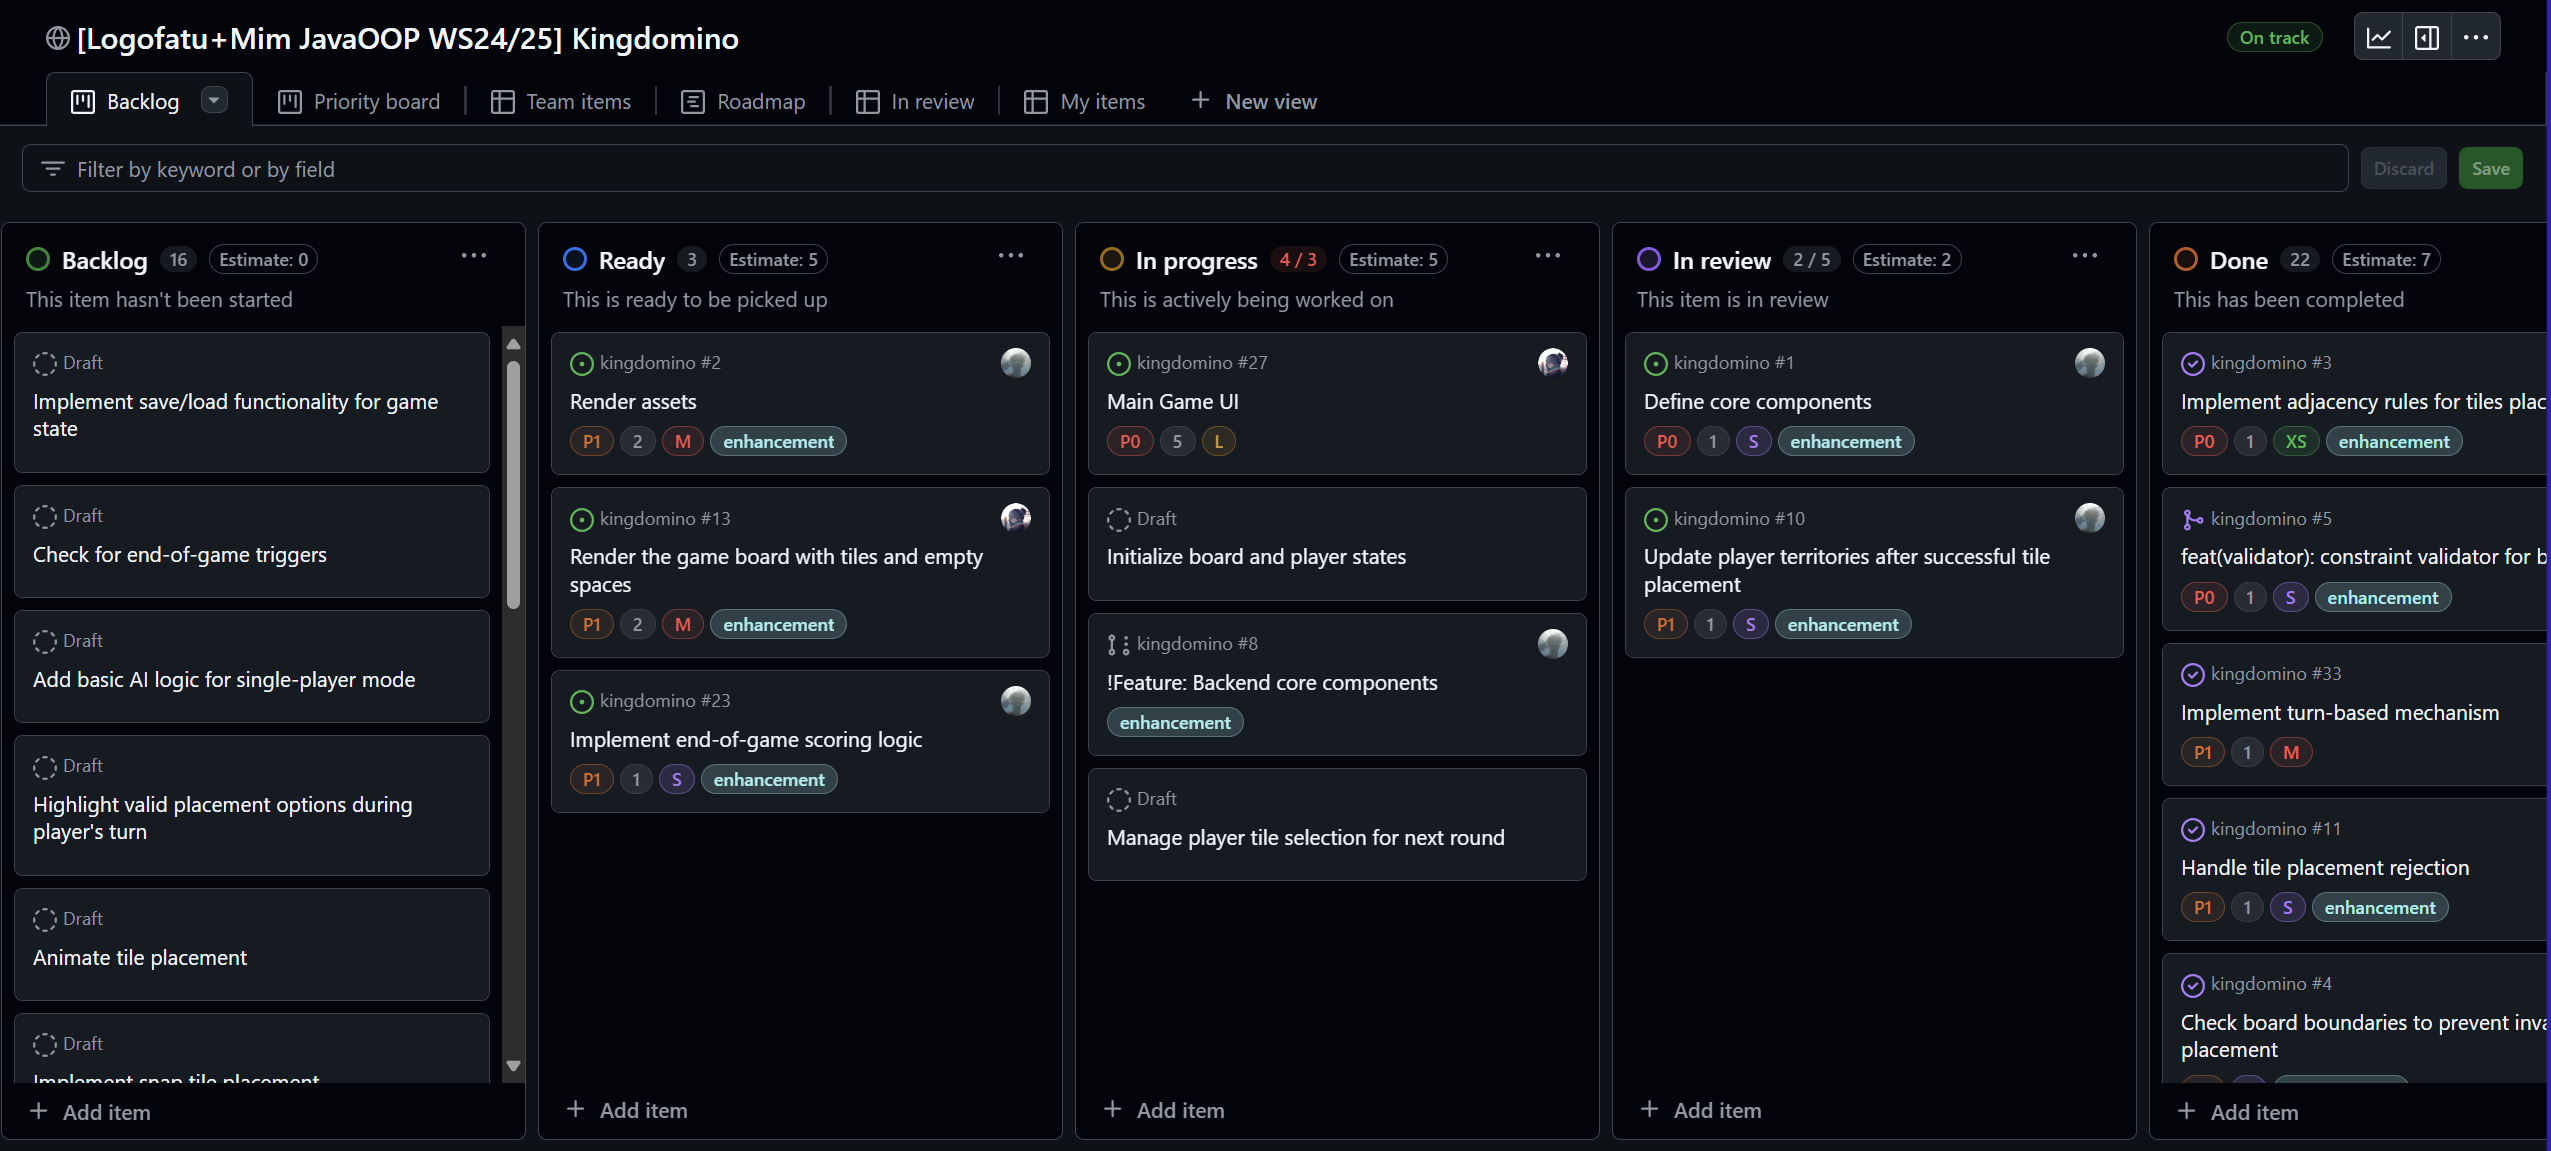
\includegraphics[width=0.48\textwidth]{assets/github-project.png}}
    \caption{Optional Process Flow Diagram (replace with your own).}\label{fig:flow_diagram}
\end{figure}

%======================================================
\section{Implementation Details}
% 6. IMPLEMENTATION DETAILS
% -- Application structure, GUI details, UML/Class Diagram, used libraries, important code snippets.

\subsection{Application Structure}
% -- High-level architecture. Possibly a diagram.

\subsection{Graphical User Interface (GUI)}
% -- Describe the interface design, layout, main widgets.

\subsection{UML/Class Diagram}
% -- Provide an overview of classes, relationships. 
%    Reference the figure in text.

\subsection{Used Libraries and Environment}
% -- Mention languages, frameworks, libraries, operating systems, version details, etc.

\subsection{Important Code Snippets}
% -- Show the relevant or tricky parts of your code with explanations.

\begin{figure}[htbp]
    % \centerline{\includegraphics[width=0.48\textwidth]{placeholder_class_diagram.png}}
    \caption{UML/Class Diagram (replace with your UML figure).}\label{fig:uml}
\end{figure}

% Example of a short code snippet:
\begin{verbatim}
// Pseudocode or short snippet
function calculateScore(board):
    score = 0
    for each territory in board:
        if territory is contiguous:
            score += territory.size * territory.crowns
    return score
\end{verbatim}

%======================================================
\section{Experimental Results, Statistical Tests, Running Scenarios}
% 7. EXPERIMENTAL RESULTS, STATISTICAL TESTS, RUNNING SCENARIOS
% -- Provide tables, charts, and discussion of the experiments you ran.

\subsection{Simulation Setup}
% -- Describe your environment, parameter choices, etc.

\subsection{Results and Evaluations}
% -- Insert tables and charts with relevant data and evaluations.

% \begin{table}[htbp]
% \caption{Example of Results Table}
% \begin{center}
% \begin{tabular}{|c|c|c|}
% \hline
% \textbf{Parameter} & \textbf{Value / Range} & \textbf{Observation}\\
% \hline
% Population Size & 50--200 & Performance improved \\
% Mutation Rate   & 5\%     & Minimal difference \\
% \hline
% \end{tabular}
% \label{tab:results}
% \end{center}
% \end{table}

%======================================================
\section{Conclusions and Future Work}
% 8. CONCLUSIONS AND FUTURE WORK
% -- Discuss overall findings, reflect on teamwork, 
%    lessons learned, and possible future improvements.

Lorem ipsum dolor sit amet, consectetur adipiscing elit.

\subsection{Team Reflection}
% -- Summarize teamwork, synergy, challenges, etc.

\subsection{What We Learned}
% -- Key lessons from implementing or analyzing the game.

\subsection{Future Development}
% -- Potential expansions, new game modes, new algorithms, etc.

%======================================================
\appendices%
\section{Gameplay Mechanic}\label{app:gameplay}
% -- Provide additional content that supports the main text.

%======================================================
% -- Follow the IEEE reference style
% -- Cite references in text, e.g., [1], [2], etc.

\bibliographystyle{IEEEtran}
\bibliography{bibliography}

\end{document}
